\documentclass[11pt]{extarticle}
\usepackage{amssymb}
\usepackage{epsfig}

\setlength{\oddsidemargin}{0.25 in}
\setlength{\evensidemargin}{-0.25 in}
\setlength{\topmargin}{-0.6 in}
\setlength{\textwidth}{6.5 in}
\setlength{\textheight}{8.5 in}
\setlength{\headsep}{0.75 in}
\setlength{\parindent}{0 in}
\setlength{\parskip}{0.1 in}

\newenvironment{Section}[2]{
  \section*{\huge{Section #1:\\ #2}}
}

\newcommand{\itab}[1]{\hspace{0em}\rlap{#1}}
\newcommand{\tab}[1]{\hspace{.2\textwidth}\rlap{#1}}

\newcommand{\lecture}[4]{
   \pagestyle{myheadings}
   \thispagestyle{plain}
   \newpage
   \setcounter{page}{1}
   \noindent
   \begin{center}
   \framebox{
      \vbox{\vspace{2mm}
    \hbox to 6.28in { {\bf 20CS6037 Machine Learning \hfill} }
       \vspace{6mm}
       \hbox to 6.28in { {\Large \hfill #1 (#2)  \hfill} }
       \vspace{6mm}
       \hbox to 6.28in { {\it Lecturer: #3 \hfill Scribes: #4} }
      \vspace{2mm}}
   }
   \end{center}
   \markboth{#1}{#1}
   \vspace*{4mm}
}

%Send your finished notes to the instructor
%({\tt ancaralescu@gmail.com}), including the Latex file and all .eps
%or .pdf files that you've created for figures. Double-check that your file compiles with {\tt pdflatex lec1.tex} before you send it.

%These notes should be complete, correct, clear, and free of typos.

\begin{document}

\lecture{MLE, MAP, Bayesian Reasoning - Chapter 3 \& 5} {Lecture 5: 9/9/14}{Anca Ralescu}{Khaldoon Ashouiliy, Kyungmook Park}

\begin{Section}{1}{Conditional Independence}
\end{Section}
\begin{Section}{2}{Transformation of Random Variables}
\end{Section}
\begin{Section}{3}{General Transformations}
\end{Section}
\begin{Section}{4}{Monte Carlo Approximation}
\end{Section}
\begin{Section}{5}{Entropy}
\end{Section}
\begin{Section}{6}{Mutual Information}
\end{Section}



\newpage

\begin{Section}{1}{Conditional Independence}
\Large{X,Y r.v. X $\perp Y$ : X and Y are independent\\\\
\underline{Def}\\
X $\perp$ Y $\Leftrightarrow$ P(X,Y) = P(X)P(Y)\\
This really means \{w $\in$ S $|$ X(w) = a\}, \{w $\in$ S $|$ Y(w) = b\}\\
are independent event for all a $\in$ Range(x); b $\in$ Range(Y)

\underline{Notation}\\
X $\perp$ Y $|$ 2 : X and Y are \textbf{\textit{Conditionally Independent} (CI)} given 2\\

P(X $\perp$ Y $|$ 2) $\Leftrightarrow$ P(X, Y $|$ 2) = P(X $|$ 2)P(Y $|$ 2)\\

\begin{figure}[htbp] %  figure placement: here, top, bottom, or page
   \centering
			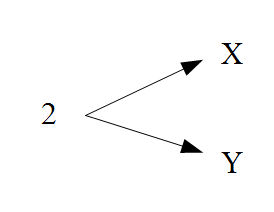
\includegraphics[width=2in]{Figure1.png}
  % \includegraphics[width=2in]{name.pdf} % uncomment this line and put the figure in the same folder as this document.
   \caption{X and Y are CI given 2}
   \label{fig:Figure1}
\end{figure}
\underline{P}(X, Y) : Joint Distribution of X and Y\\
\{w $\in$ S $|$ X(w) = a\}, \{w $\in$ S $|$ Y(w) = b\}\\
Can extend to \underline{P}(X$_1$, $\ldots$ , X$_D$) : CDF, PDF/PMF\\
\itab{COV(X, Y)} \tab{$\triangleq$ E[(X-E(X))(Y-E(Y))]}\\
\itab{}\tab{ = E[XY - XE(Y) - YE(X) + E(X)E(Y)]}\\
\itab{}\tab{ = E(XY) = E(X)E(Y)}\\

\newpage

}
\end{Section}
\begin{Section}{2}{Transformation of Random Variables}
\end{Section}
\begin{Section}{3}{General Transformations}
\end{Section}
\begin{Section}{4}{Monte Carlo Approximation}
\end{Section}
\begin{Section}{5}{Entropy}
\end{Section}
\begin{Section}{6}{Mutual Information}
\end{Section}

\end{document}

